\documentclass[11pt,leqno]{article}
\usepackage[noend]{algorithmic}
%\usepackage{algorithm}% http://ctan.org/pkg/algorithms
%\usepackage{algpseudocode}% http://ctan.org/pkg/algorithmicx
\usepackage{pgfplots}
\usepackage{tikz}
\pgfplotsset{width=7cm,compat=1.12}
\usepackage{verbatim}
\usepackage[noend]{algorithmic}
%\usepackage{algorithm}% http://ctan.org/pkg/algorithms
%\usepackage{algpseudocode}% http://ctan.org/pkg/algorithmicx
\usepackage{tabularx}
\usepackage{amssymb}
\usepackage{amsmath}
\usepackage{latexsym}
\usepackage{mathrsfs}
\usepackage[export]{adjustbox}
\usepackage{xcolor}
%\usepackage{yhmath}
\usepackage{amsthm}
\usepackage{mathrsfs}
\usepackage{hyperref}
\usepackage{comment}
\usepackage{graphicx}
\usepackage{hyperref}
\usepackage{tikz}
\usepackage{pgfplots}
\usepackage{placeins}
\usepackage{ulem}
\usepackage{datetime}
%\usepackage{kpfonts}
\usepackage{float}
\usepackage{changepage}
\usepackage{arydshln}
\usepackage{array}
\usepackage{xcolor}
%\usepackage{yhmath}
\usepackage{amsthm}

\makeatletter
\def\hlinewd#1{%
	\noalign{\ifnum0=`}\fi\hrule \@height #1 %
	\futurelet\reserved@a\@xhline}
\makeatother

\begin{document}
\centerline{\bf \Large Problema comis-voiajorului, }
\centerline{\bf \ utiliz\^ and un Algoritm Genetic \c si algoritmul lui Christofides.}
	
\vspace{0.5cm}
\centerline{\author MModoranu Cosmin, grupa A6, anul II}
\centerline{\author  DD\u ar\u ab\u aneanu Cosmin, grupa A6, anul II}

\vspace{0.5cm}
\centerline{Ianuarie, 2021}
\section{Abstract}
Problema comisului-voiajor  este o problem\u a NP-dificil\u a \c si important\u a \^ in domeniul distribu\c tiei \c si a  logisticii. Acest document ofer\u a informa\c tii legate de doi algoritmi utiliza\c ti \^ in rezolvarea PCV-ului \c si mai ofer\u a rezultate care eviden\c tiaz\u a acurate\c tea  m\u arita a algoritmului genetic fa\c t\u a de cea a algoritmul lui Cristofides \c si diferen\c ta de viteza de rulare a algoritmului lui Christofides care a rulat mult mai repede fa\c t\u a de algoritmul genetic.  

\section{Introducere}
Problema comisului-voiajor(PCV) este  o problem\u a  bine cunoscut\u a \c si important\u a \^ in optimizarea combinatorial\u a.Scopul este de a g\u asi drumul cel mai scurt ce viziteaz\u a fiecare ora\c s dintr-o  list\u a dat\u a, cate o singur\u a dat\u a, \^ drum care  se \^ intoarce la ora\c sul din care a plecat.
Se eviden\c tiaz\u a diferen\c tele de performan\c t\u a utiliz\^ and algoritm genetic \c si o euristic\u a numit\u a Algoritmul lui Christofides.

 \par Rezolvarea PCV este o parte important\u a  fiind utilizat\u a \^ in multe aplica\c tii  precum rutarea vehiculelor, cablarea computerelor, \^ in organizare, des \^ intalnit\u a  \^ in re\c tele de comunica\c tii .


\subsection{Descrierea problemei}

Distan\c ta total\u a a unei solu\c tii poate fi exprimat\u a \^ in felul urm\u ator:
$$ T_d=\sum_{i=1}^{n-1}d(V_i,V_{i+1})+d(V_n,V_1), $$ unde  $Path(\pi)$= $\{ V_1,V_2,...,V_n \}$ este o permutare a ora\c selor $\{1,2,...n\}$ \c si $ d(V_i,V_{i+1}) $ reprezint\u a distan\c ta de la ora\c sul $V_i$ la ora\c sul $V_j$.

Se cere determinarea unui drum   de lungime  minim\u a \^ in care fiecare ora\c s este vizitat o singur\u a dat\u a. 

 
\section{Metode}

\subsection{Algoritm genetic}

Un \uline{Algoritm genetic} : este o metodă ce are ca surs\u a de inspira\c tie evolu\c tia biologic\u a \c si utilizeaz\u a un vocabular \^ imprumutat din genetic\u a.\\
Sunt algoritmi ce \^ imbun\u at\u a\c tesc solu\c tia pas cu pas de-a lungul mai multor genera\c tii.\\
Pentru rezolvarea problemei vom defini urm\u atoarele  elemente:\\
-o reprezentare a solu\c tiilor candidat;\\
-o procedur\u a de ini\c tializare a popula\c tiei ini\c tiale  de solu\c tii candidat;\\
-o func\c tie de evaluare(func\c tia fitness); \\
-o schem\u a de selec\c tie;\\
-crossover ;\\
-operatorii genetici ;\\
Astfel:\\
Reprezentarea solu\c tilor este facut\u a printr-un vector de numere intregi ce reprezint\u a ordinea parcurgerii ora\c selor. Este o permutare a elementelor \^ intre 0 si $n-1$ pentru n ora\c se.
. Se extrag coordonatele din unele instan\c te din libr\u aria TSPLIB \cite{TSPLIB} si se calculeaza matricea de cost adiacent\u a care e folosit\u a de-al lungul algoritmului.
 \\
 \textbf{Funcția fitness} : Fitness-ul unei solu\c tii se calculeaz\u a ca fiind 
$$ \mathbf{ f(x) = distanta\_tur(x) + 0.0001}$$
Se urm\u areste minimizarea acesteia pe parcursul algoritmului genetic.
\\
\par \textbf{TournamentSelection} 
Alegem \textit{k} soluții  din popula\c tia actual\u a \c si \^ il alegem ca rezultat cel mai bun dintre acestea.

\par \textbf{RankSelection}: Se sorteaza solu\c tiile dup\u a fitness \c si se atribuie fiec\u areia o probabilitate de a fi aleas\u a propor\c tional\u a cu indecsul pe care se afl\u a.

\par \textbf{RouletteWheelSelection}: Calcul\u am valoarea fitness pentru toate solu\c tiile \c si le atribuim fiec\u arei din ele o probabilitate care reflect\u a c\^ at de bun\u a este \^ in compara\c tie cu altele, pentru o soluție mai bu\u a se va ob\c tine o probabilitate mai mare ca aceasta s\u a fie aleas\u a.

\par \textbf{Crossover} : Aplic\^ and Crossover peste dou\u a solu\c tii din popula\c tie ob\c tinem o nou\u a solu\c tie pe care o vom numi fiu. Se alege o t\u aietur\u a aleatorie. Prima parte p\^ an\u a la t\u aietur\u a se men\c tine \^ in fiu \c si apoi se completeaz\u a cu ora\c sele din a dou\u a solu\c tie \^  in ordinea \^ in care acestea apar.Fiul \^ i\c si completeaz\u a lista ora\c selor din a dou\u a solu\c tie doar dac\u a aceste solu\c tii  nu se g\u asesc printre datele pe care fiul le are deja.

\textbf{Mutatie}: Se efectueaza prin \textbf{rotire} \c si \textbf{interschimbare}.
\\
\textbf{Interschimbarea}: Se aleg doua pozi\c tii din solu\c tia pe care aplic\u am operatorul \c si se interschimb\u a valorile de la pozi\c tiile respective.
\\
\textbf{Rotirea}: Similar cu std::reverse. Alegem dou\u a pozi\c tii \^ in cadrul solu\c tie pe care aplic\u am operatorul \c si rotim elementele dintre cei doi indec\c si adic\u a primul element o s\u a fie interschimbat cu ultimul, al doilea element o s\u a fie interschimbat cu penultimul \c s.a.m.d.
\\
 
\subsection{Algoritmul lui Christofides}
\uline{Algoritmul lui Christofides}: Algoritm care ne ajuta s\u a g\u asim solu\c tii pentru PCV \^ in instan\c te care verific\u a inegalitatea triunghiular\u a. Este potrivit pentru c\u a lucr\u am cu coordonate 2D \c si se respect\u a constrangerea aceasta. Este o schem\u a de aproximare \^ in timp polinomial care garanteaz\u a ca solu\c tiile sunt m\u acar sub $\frac{3}{2}$ din optim.  Pentru a g\u asi o solu\c tie pentru PCV \c si prin acest algoritm se parcurg urmatorii pa\c si:
\\
1. Se gase\c ste un arbore par\c tial de cost minim \textbf{T}.
\\
2. Se formeaz\u a mul\c timea \textbf{O} ce con\c tine nodurile impare din \textbf{T}.
\\
3. Se g\u ase\c ste un cuplaj perfect \textbf{M} \^ in subgraful indus de nodurile din \textbf{O}
\\
4. Se combin\u a muchiile lui \textbf{M} si \textbf{T} pentru a forma un multigraf \textbf{H} unde fiecare nod are grad par.
\\
5. Se formeaz\u a un circuit Eulerian din \textbf{H}.
\\
6. Se transform\u a \^ in circuit Hamiltonian prin reducerea nodurilor care se repet\u a (se iau scurt\u aturi).

\section{Descriere experimente}

\begin{flushleft}
Se ruleaz\u a Algoritmul Genetic \c si Algoritmul lui Christofides pe 6 instan\c te cunoscute ale problemei. Algoritmul genetic a fost  rulat de $n=30$ ori \c si se \^ inregistreaz\u a date precum cea mai bun\u a solu\c tie, media solu\c tilor \c si cea mai slab\u a solu\c tie.\\
Parametrii AG-ului sunt urm\u atorii:\\
POP\_SIZE = 1000 ; $P_{CX} = 0.2$ ; $P_{M} = 0.05$ ; MAX\_GENERATIONS = 3000

\end{flushleft}

\section{Rezultate experimentale}

	\begin{figure}[H]
		
		\begin{adjustwidth}{-50pt}{}
\begin{tabular}{|l|c|c|c|c|c|c|c|}
	\hline
	Algoritm & Num\u ar ora\c se & Instanta & Worst result & Average result & Best result & Optim   & Avg. time (s) \\ \hline 
	AGE      & 76                & eil76    & 619.295      & 562.275        & 553.414     & 538     & 32s           \\ \hline
	AGE      & 198               & d198     & 16821.7      & 16549.2        & 16463       & 15780   & 90s           \\ \hline
	AGE      & 318               & lin318   & 53192.3      & 49233.7        & 48213.2     & 42029   & 211s          \\ \hline
	AGE      & 70                & st70     & 695.4        & 687.53         & 686.2       & 675     & 24s            \\ \hline
	AGE      & 225               & tsp225   & 4453.18      & 4376.65        & 4291.3      & 3919    & 149s           \\ \hline
	AGE      & 280               & at280    & 3021.3       & 2943.63        & 2873.2      & 2568.88 & 166s           \\ \hlinewd{1.5px}
	AC       & 76                &  eil76        & 670.45       & 670.45         & 670.45      &   538      & 1s            \\ \hline 
	AC       & 198               &  d198        & 18183.4      & 18183.4        & 18183.4     & 15780        & 2s            \\ \hline
	AC       & 318               &  lin318        & 57608        & 57608          & 57608       &  42029       & 2s            \\ \hline
	AC       & 70                  &   st70       &     842.3         &     842.3            &    842.3          &  675        &  1s             \\ \hline 
	AC       & 225                  &  tsp225       &      5145.24           &     5145.24           &   5145.24             & 3919        &   2s             \\ \hline
	AC       & 280                  &   at280      &     3405          &    3405            &    3405          &  2587.88       &  2s              \\ \hline
\end{tabular}

			
		\end{adjustwidth}
		
		\caption{Un set de date ob\c tinute cu ajutorul unui Algoritm Genetic si a algoritmului lui  Christofides.}
	\end{figure}

	\begin{figure}[H]
	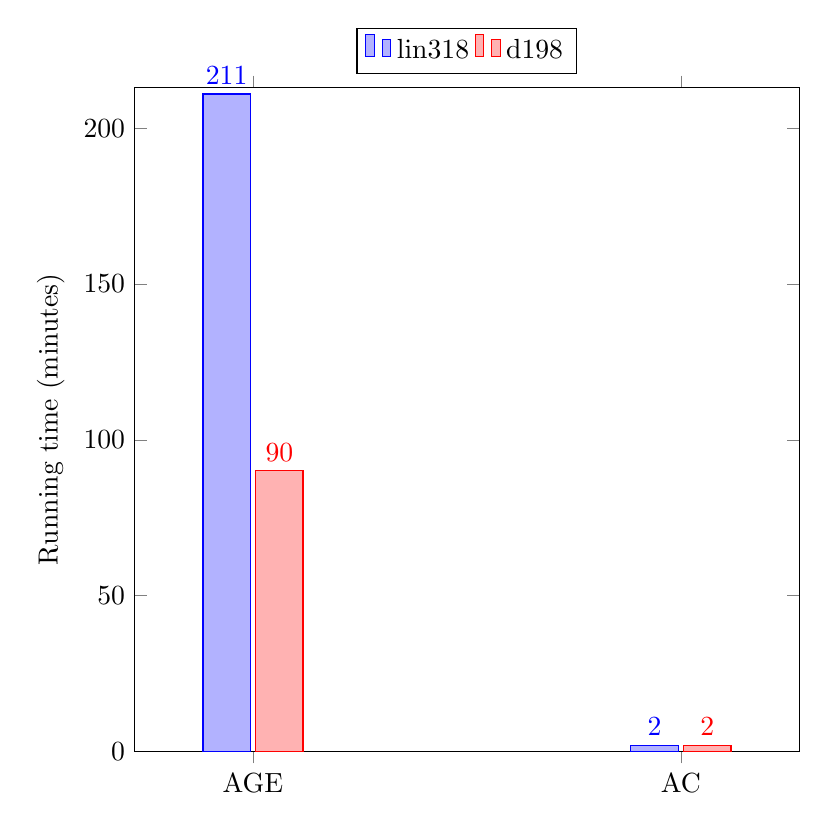
\begin{tikzpicture}
		\pgfplotsset{%
			width=1\textwidth-60,
			height=1\textwidth-60
		}
		\begin{axis}[
			ybar,
			enlargelimits=0.01,
			legend style={at={(0.5,1.09)},
				anchor=north,legend columns=-1},
			ylabel={Running time (minutes)},
			symbolic x coords={AGE,AC},
			xtick=data, 
			bar width=0.6cm,
			enlarge x limits={abs=1.5cm},
			nodes near coords,
			nodes near coords align={vertical},
			]
			\legend{lin318,d198} 
			\addplot coordinates {(AGE,211)(AC,2)  };
		\addplot coordinates {(AGE,90)(AC,2)  };
		
 	
		\end{axis}

	\end{tikzpicture}
\caption{Grafic ce reprezint\u a timpul mediu al instan\c telor d198 \c si lin318 utiliz\^ and AGE \c si AC.}
	\end{figure}




\section{Interpretarea rezultatelor}
Din punct de vedere al timpului de execu\c tie algoritmul genetic ofer\u a rezultat mult mai lent fa\c t\u a de algoritmul lui Christofides. Rezultatele ob\c tinute de algoritmul genetic sunt  mult mai precise fa\c t\u a de rezultatul ob\c tinut de algoritmul lui Christofides dar \^ in schimb AC a rulat foarte repede(1-3s). De exemplu pentru instan\c ta lin318 pentru AG rezultatul a fost 49233 vs 57600 pentru AC \^ in condi\c tiile \^ in care algoritmul \^ incepe cu prima genera\c tie la valoarea 400000 \c si optimizeaz\u a pe parcursul rul\u arii un rezultat cu 345000 mai mic.
	
\section{Concluzii}
Algoritmul genetic a fost mai bun pentru calitatea raspunsurilor oferite \c si este mai potrivit c\^ and se cere optimizarea solu\c tiei c\^ at mai mult, c\^ at mai aproape de optim.
Algoritmul lui Christofides func\c tioneaz\u a mai bine pe num\u ar mare de orase din cauza rapidit\u a\c tii acestuia. Pentru num\u ar mai mic de ora\c se ($\le 300$) este mai potrivit algoritmul genetic
precum diferen\c ta de timp(in medie 200 secunde) nu este a\c sa mare. Algoritmul lui Christofides folose\c ste mai mult\u a memorie pentru stocarea MST-ului \c si a grafurilor ob\c tinute la fiecare pas dar
din cauza timpului mic de rulare remarc\u am c\u a nu sunt \c tinute \^ in memorie prea mult.

\par Proiectul se afla la : \url{https://github.com/KenKQDEs/Genetic-Algorithm-TSP/commits/develop?fbclid=IwAR2fnuXLVNRkuoBwt9fd2ScdxSaQp-8zkuPhJ_2_ahX5WF2rH7AnzBNfpEs}

\begin{flushleft}

\end{flushleft}
\section{Bibliografie}
\begin{thebibliography}{9}

\bibitem{  Pagina laboratorului:}
Pagina laboratorului:
\url{https://profs.info.uaic.ro/~eugennc/teaching/ga/}




\bibitem{Universitatea "Alexandru Ioan Cuza"}
  Documentație.Algoritmi Genetici:
\url{http://students.info.uaic.ro/~vladut.ungureanu/Algoritmi-genetici-ID.pdf}


\bibitem{Raport stintific}
 Raport stintific.Autor: Chih-Cheng Hung\\ Informații utile despre  algoritmul genetic utilizat  pentru TSP
 simetric:
  \url{https://www.hindawi.com/journals/mpe/2015/212794/?fbclid=IwAR2p3Mp8c2ClB562FWm2O4d5oieIcUGamZUPc_WjV3xte_Nd17Pb9NPSh0k}

\bibitem{Raport stintific}
 Raport stintific.Autor:Xiao Yan Yun\\ Raport stintific despre TSP.
  \url{https://www.scientific.net/AMR.694-697.2901}

\bibitem{ Informatii PCV}
  Informatii PCV:
  \url{https://ro.wikipedia.org/wiki/Problema_comis-voiajorului#Algoritmul_lui_Christofides_pentru_PCV}

\bibitem{Documentatie PCV}
Documentatie.Problema comis-voiajorului:
\url{https://www.geeksforgeeks.org/travelling-salesman-problem-set-2-approximate-using-mst/}

\bibitem{Documentatie AC}
Documentatie.Algoritmul lui Christofides:
\url{https://youtu.be/M5UggIrAOME}

\bibitem{Informatii AC}
Documentatie.Algoritmul lui Christofides:
\url{https://en.wikipedia.org/wiki/Christofides_algorithm}

\bibitem{TTutorial youtube}
  Documentație.Problema comis-voiajorului:
\url{https://www.youtube.com/channel/UCzvWh64GQm_OfkJXyYo7whQ}

\bibitem{ Documentatie Latex}
  Documentatie Latex:
  \url{https://www.latex-project.org/help/documentation/}

\bibitem{TSPLIB}
TSPLIB:
\url{http://comopt.ifi.uni-heidelberg.de/software/TSPLIB95/}



\end{thebibliography}  


\end{document}
